\chapter{Introduction}
To start this thesis a motivation for this scientific work is given. Then, the required knowledge is presented. After the presentation of the basic knowledge the objective of this bachelor thesis is displayed. To close this chapter an outline of this paper is given in the last section.

\section{Motivation}
One of several requirements regarding complex life is cell adhesion. If cells do not stick to each other the only living things would be cells. 
In humans and animals, organs and epithels are made of several cells and several layers of cells. This is also the case for the urothelium, which is an epithelium, i.e. a membranous tissue which consists of one or several layers. For the urothelium it is necessary that the cells stick to each other. Otherwise the functions of the urothelium could not be executed and also it would not be able to grow.

There are two types of tumors. One is the benign and the other one is the malignant tumor \cite{Poplawski2009}. The benign tumor is self limited. Thus, it does not invade surrounding tissues, nor does it spread into other body parts \cite{Poplawski2009}. The malignant tumor on the other hand is not limited in its growth and is able to invade other body parts \cite{Poplawski2009}. 

Since bladder cancer is one of the most common cancer types among men it is important to understand how and why the cancer is able to grow. \newline
Bladder cancer starts to grow in the urothelium. With its growth and spread, the structure of cells sticking together changes. In this case, the urothelium is no longer able to completely perform its tasks. In order to understand the urothelium, how and when bladder cancer appears, it is necessary to observe the epithel.

To understand the functionalities of organs and epithels, in general organisms, observations are essential. For the urothelium this is already done as there are several in vitro experiments about the methodology of the urothelium \cite{WRCross2005, PuneetKhandelwal2009}. After an observation of an epithel or organ is complete, researches are able to predict how the observed organism will react in different situations. To verify these predictions a simulation is necessary. A simulation is an abstract illustration of the reality, but it can also be used to change reality in a for the research specific way, to get more knowledge of the epithel, or an organism in general.

A simulation should always be as simple as possible but not too simple. Otherwise the simulation does not represent the reality. 
There are several programs with different algorithms for cell simulation. A popular approach is the \ac{GGH} model. This model is popular because it is easy to describe how cells interact with each other and it is possible to define constraints for the volume and surface of each cell. \newline
The program \ac{CC3D} is a simulation program, which uses the \ac{GGH} algorithm in its simulation. In the moduro project \ac{CC3D} is used, and with the program the \ac{GGH} algorithm is used.

The target of the moduro project is to predict under which circumstances bladder cancer occurs and when it is able to grow. Therefore, 16 different morphogenesis models of the urothelium were created. An overview of these models is displayed in table \ref{tbl:16Models} at page \pageref{tbl:16Models}. So far, all 16 models were simulated in 2D for a timespan of 720 days. The results reveal that some of the models are more realistic than others.

A 2D simulation of the urothelium might not give as many aspects as a 3D simulation could do, because a cell is a three dimensional organism. Thus, the aim of this bachelor thesis is to create a 3D simulation of these 16 different models. With this 3D simulation it is hoped to receive new insights into the urothelium and how bladder cancer occurs.

\section{Background}
\subsection{Biology of the Urothelium}
Bladder cancer is the fourth most common cancer type in men  according to everydayhealth.com \cite{EveryDayHealth.com}. Bladder cancer usually starts with some cells in the bladder growing uncontrolled. From these cells the tumor can spread further into surrounding areas \cite{Cancer.org}. The most common bladder cancer type is urothelial carcinoma \cite{Cancer.org}.

The bladder is located in the lower urinary tract and consists of several parts. The urothelium is one part of it and coats the bladder \cite{Lazzeri2006}. More specifically, it covers the bladder from the renal pelvis to the proximal urethra \cite{Yamany2014, Birder2005}.

Two important tasks of the bladder are the storage and release of urine. To do so the bladder will extend, during the storage, and then shrink again \cite{Karl-ErikAndersson2004}. One task of the urothelium is to form a distensible barrier \cite{Apodaca2004, Lazzeri2006, PuneetKhandelwal2009, Lewis2000, WRCross2005}, which prevents unregulated exchange of ions, solutes, and toxic metabolites between the bladder and the blood \cite{Apodaca2004, Lazzeri2006, PuneetKhandelwal2009, Lewis2000}. The urothelium ensures its barrier function through enlargement and downsizing of its size. This is done by the largest cells of the urothelium, the umbrella cells, also called superficial cells. Since the umbrella cells are in direct contact with the bladder it is their task to change size and form during the growth and shrink process of the bladder. Birder \cite{Birder2005} described the urothelium as “… a responsive structure capable of detecting physiological and chemical stimuli and releasing a number of signaling mole-cules.”. Another task of the urothelium is to control the movement and passage of macromolecules, ions, water, toxic metabolites and solutes \cite{Apodaca2004, PuneetKhandelwal2009}. If the urothelium is damaged, it rapidly generates new cells, to ensure full functionality \cite{Apodaca2004, Yamany2014, PuneetKhandelwal2009}.

To receive a better overview of the different cell types, they are explained in the following paragraph. In figure \ref{img:physiology_urothelium} a simplified illustration of the urothelium with its different cell types and cell layers is provided. \newline
The umbrella cells are connected directly with the bladder and have an average diameter of 25 up to \SI{250}{\micro\metre} \cite{Yamany2014, PuneetKhandelwal2009}. 

Below these cells the intermediate cells are located, with an average diameter of 10 up to \SI{20}{\micro\metre} \cite{Yamany2014, PuneetKhandelwal2009}. There are at least three and up to five layers of the intermediate cells \cite{PuneetKhandelwal2009}. 

The smallest and the most common cells in the urothelium are the basal and stem cells. Those cells have a diameter of up to \SI{10}{\micro\metre} \cite{Lazzeri2006, PuneetKhandelwal2009}. 

The urothelium consists of several layers. In the first layer, there are the basal and stem cells. Above them, there are several layers of intermediate cells. On top of the epithelium is one layer of umbrella cells.


\begin{figure}[th]
	\center
	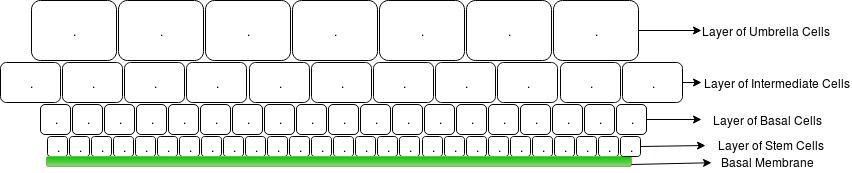
\includegraphics[scale=0.3]{figures/Urothelium.png}
	\caption[A simplified illustration of the urothelium]{A simplified illustration of the urothelium. At the very bottom is the basal membrane. Above the membrane the stem and basal cells are displayed. The blue cells represent the stem cells, the red cells display the basal cells. Above the layer out of these two cell types, the urothelium contains several layers of intermediate cells. At the top of the urothelium is a layer of umbrella cells.}
	\label{img:physiology_urothelium}
\end{figure}

\subsection{CompuCell3D}
\ac{CC3D} is an open-source program, which provides a simulation environment for multi- or single-cell-based modeling of tissues, organs and organisms \cite{CC3D.org}. To do so, \ac{CC3D} uses the \ac{GGH} model in its simulation. 
CC3D provides the possibility to create programs for the simulation, e.g. cell growth, mitosis, apoptosis or necrosis scripts, in Python, C++ or in CC3DML, which is their own Markup Language. With such programs CC3D allows the user to modify the behavior of the simulation for a specific purpose.
CC3D uses the \ac{GGH} approach, which is explained in the next section. It allows the user to choose between two cell-lattice types, i.e. a presentation of the pixels or voxels, i.e. a pixel with three dimensions, of a cell at a specific position in the simulation field. By default, it uses a square-lattice of single pixels for each dimension, an example therefore is displayed in figure \ref{img:2DSquareLattice}. \ac{CC3D} provides the possibility to use a hexagonal-lattice, where the pixels are hexagons in two dimensions, or rhombic dodecahedrons in three dimensions.
The core of a \ac{GGH} simulation is the effective energy \cite{MaciejH.Swat2017}, \ac{CC3D} tries to minimize this effective energy every \ac{MCS}, i.e. a calculation step in the simulation. The basic form for the effective energy is:

\begin{equation}
\mathcal{H}_{boundary} = \sum_{\vec{i},\vec{j}}^{ }{J(\tau(\sigma(\vec{i})),(\tau(\sigma(\vec{j})))(1-\delta(\sigma(\vec{i}),(\sigma(\vec{j})))}
\end{equation}
This equation is a part of the equation of the \ac{GGH} model. This model is explained in the next section. It is possible to extend this form in two ways. Either a volume or a surface constraint for each cell can be added. 
During each \ac{MCS} an index-copy attempt takes place \cite{MaciejH.Swat2017}. In this index-copy attempt a pixel is selected, and it is tried to overwrite a randomly chosen pixel, next to the current pixel. It succeeds and takes place if this index copy attempt decreases the effective energy \cite{MaciejH.Swat2017}. Each \ac{MCS} \ac{CC3D} tries to minimize the effective energy with index copy attempts. 

\begin{figure}[th]
	\center
	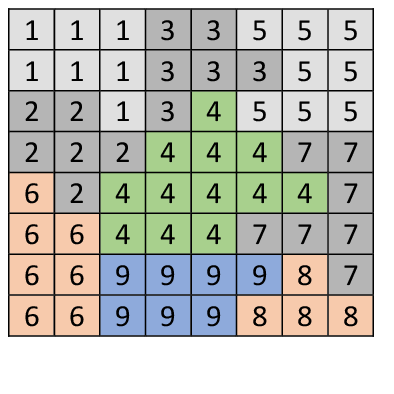
\includegraphics[scale=0.4]{figures/2DSquareLattice.png}
	\caption[A two dimensional square lattice]{A square lattice in 2D. The same digits represent one cell $(\sigma(\vec{i}))$, whereas the different colors represent different cell types $\tau(\sigma)$.}
	\label{img:2DSquareLattice}
\end{figure}

\subsection{Glazier Graner Hogeweg Model} \label{subsec:Intro_GGH}
Glazier and Graner developed several formulas and models which are presented in this subsection with focus on the \ac{CPM} and \ac{GGH} model.\newline
The \ac{GGH} model is widely used in biological simulations, since it provides a good flexibility, extensibility and usability \cite{Glazier2007}. 
Glazier and Graner \cite{Glazier2007} developed the \ac{EPM} as an extension of the large-q Potts model, which itself is an extension of the Ising Model. Nowadays, this model is called \ac{CPM} \cite{Glazier2007, Graner1992, Glazier1993}. Glazier and Graner extended the \ac{CPM} in a way that also volume constraints are considered for the Hamiltonian, i.e. the effective energy, as it is displayed in the following equation:

\begin{equation}\label{eq:H_CPM}
\begin{split}
\mathcal{H}_{CPM} & = \sum_{\vec{i},\vec{j}}^{ }J(\tau(\sigma(\vec{i})),(\tau(\sigma(\vec{j})))(1-\delta(\sigma(\vec{i}),(\sigma(\vec{j}))) \\
		 & + \sum_{\sigma}^{}{\lambda_{vol}((\tau)v(\sigma)-V_{target}(\tau(\sigma)))^2}
\end{split}
\end{equation}
The Hamiltonian of equation \ref{eq:H_CPM} describes the effective energy for the extension of the \ac{CPM} model. The first sum describes $J$ of all cells, the adhesion energy between different cells. Therefore, every cell has a specific cell type $\tau(\sigma)$ \cite{Glazier1993, Graner1992}. Each cell is placed onto a lattice with a spin $(\sigma(\vec{i}))$ for every given dimension \cite{Graner1992, Glazier2007}. The adhesion energy between cells is only considered if the Kronecker delta is 0. Thus, the adhesion energy between cells is considered if $\delta(\sigma, \sigma') = 0$ \cite{Glazier1993, Graner1992, Stott1999, Glazier2007, Chen2007, Cickovski2005}. \newline
With the second sum over all cells the volume of each cell is now considered within the effective energy. The user is now able to set a target volume $V_{target}(\tau(\sigma))$ for each cell and a multiplier $\lambda_{vol}$ for the deviation between the current volume $(\tau)v(\sigma)$ and the target volume. During the simulation this deviation is tried to be kept as small as possible for every cell in order to keep the effective energy as small as possible.

Together with Hogeweg Glazier and Graner further developed the created extension of the \ac{CPM}. The further developed model is called \ac{GGH} model. The main extension is that the user is now able to add surface area constraints \cite{Graner1992, Glazier1993, Glazier2007} as well as to use a negative boundary energy \cite{Glazier2007}. With the surface constraint the equation for the effective energy of the \ac{GGH} model is:

\begin{equation}\label{eq:H_GGH}
\begin{split}
\mathcal{H}_{GGH} & = \sum_{\vec{i},\vec{j}}^{ }J(\tau(\sigma(\vec{i})),(\tau(\sigma(\vec{j})))(1-\delta(\sigma(\vec{i}),(\sigma(\vec{j}))) \\
		 & + \sum_{\sigma}^{}{\lambda_{vol}(\tau)v(\sigma)-V_{target}(\tau(\sigma)))^2} \\
		 & + \sum_{\sigma}^{}{\lambda_{sur}(\tau)s(\sigma)-S_{target}(\tau(\sigma)))^2}
\end{split}
\end{equation}
In addition to the Hamiltonian of equation \ref{eq:H_CPM} is the surface constraint. It has the same principle as the volume constraint. Thus, the user is able to define a target surface $S_{target}(\tau(\sigma))$ for each cell and a multiplier $\lambda_{sur}$ for the deviation between the target and the actual surface $(\tau)s(\sigma)$ of each cell. Since the volume and surface constraint are included in the effective energy, it should be possible to use these two parts of the effective energy to shape the cells.


Beside the surface constraint the new model allows the user to model (a): cell growth and proliferation (b): mitosis, i.e. cell division (c): fields, forces and diffusion and (d): chemotaxis and haptotaxis \cite{Glazier2007}. \newline
Glazier et. al. describe their models as: 
\begin{quote}
"GGH models define biological structure consisting of the configuration of a set of \textit{generalized cells}, each represented on a \textit{cell lattice} as a domain of lattice sites sharing the same cell index [...], a set of \textit{internal cell states} for each cell [...], and a set of \textit{auxiliary fields} ...” \cite{Glazier2007}.
\end{quote}

“Initial conditions emulating a particular biological configuration rather than random initial conditions.” \cite{Glazier2007} brings the advantage that the \ac{GGH} model now has biologically motivated properties instead of physically motivated properties \cite{Glazier2007}.



\section{Objective}
The aim of this bachelor thesis is to create a 3D morphogenesis simulation of the urothelium using \ac{CC3D}.  The task is to modify the current application, of the 2D simulation, in a way that this program can be used for a 3D simulation, because the simulation models and the program for a 2D simulation are given and the simulation is done by \ac{CC3D}. \newline
The required changes are all in the program, because the models of the 2D simulation should be also used for the 3D simulation.
Therefore, some parts of the program have to be modified whereas other parts have to be developed. It is possible to try to let the cell have a different shape than in the 2D simulation, because a third dimension will be added to the simulation.
The result of this bachelor thesis will be presented with an analysis of a 3D simulation. A model therefor is selected out of the models which were created earlier in the project. These models are explained in section \ref{sec:Models}.


\section{Outline}
Chapter 'State of the Art' provides the status at which the project was at the beginning of this bachelor thesis. Once the basic knowledge and the 'State of the Art' are explained, the modifications in the program during this journey are revealed in chapter 'Methods'. Then, in chapter 'Results' the outcome of this thesis is presented. After the results are presented, they are discussed of different perspectives in chapter 'Discussion'. In chapter 'Future Work' ideas for the future of the project are presented and to round up this paper a conclusion is provided in chapter 'Conclusion'.